\section{Aire de contact}

\subsection{Tribologie, science des frottements}

La rugosité des faces en contact crée de l'adhérence. Au niveau microscopique, comme illustré à la figure~\ref{contact_entre_2_solides}, les atomes des deux solides sont interaction --- liaison chimique, force de Van Der Waals--- appliquant une force supplémentaire perpendiculaire à la surface moyenne de contact. Frottement statique, Force de décrochage, adhésion.\par
 
\begin{figure}[!h]
\begin{center}
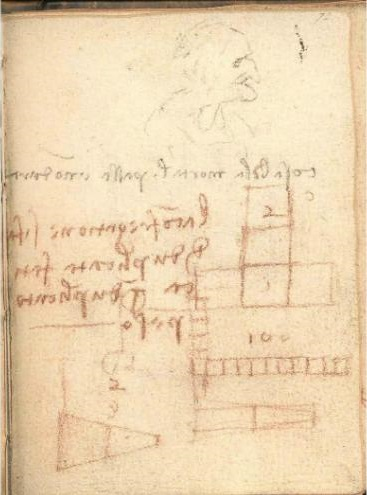
\includegraphics[width=0.7\textwidth]{Photos/LeonardDeVinci_friction_1} 
\end{center}
\caption{Illustration du contact réel entre deux solides --- défauts microscopiques sur la surface des solides.}
\label{contact_entre_2_solides}
\end{figure}

Frottement dynamique, énergie libéré lors de la rupture des liaisons.  

Origine de la tribologie, Travaux de Leonard De Vinci (1452-1519). Vers 1480, il énonce la loi suivante traduite en français “La friction double l’effort quand le poids double” (\textit{“La confregazione si fa di duplicata fatica in duplicato peso”}), image de l'archive à la figure~\ref{LeonardDeVinci}~(a). Ainsi, appuyer par d'autres dessins, présent à la figure\ref{LeonardDeVinci}~(b), il est supposé que Leonard De Vinci savait que “la force de frottement agissant entre deux surfaces qui glissent est proportionnelle à la charge qui pousse les surfaces l’une contre l'autre et que la friction est indépendante de la surface apparente de contact entre les deux surfaces”. Ce qui devancerait les travaux du physicien français Guillaume Amontons (1663-1705) qui était à l’origine de cette théorie en 1699.\par
\begin{figure}[!h]
\begin{center}
a)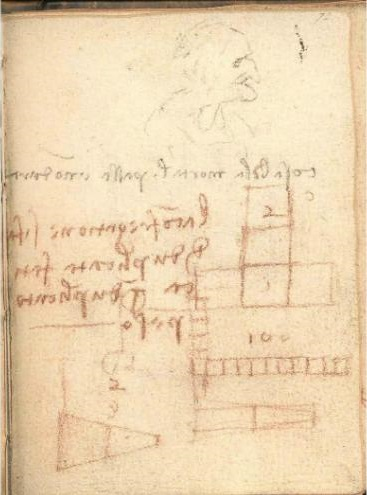
\includegraphics[width=0.45\textwidth]{Photos/LeonardDeVinci_friction_1}\hspace{0.5mm}
b)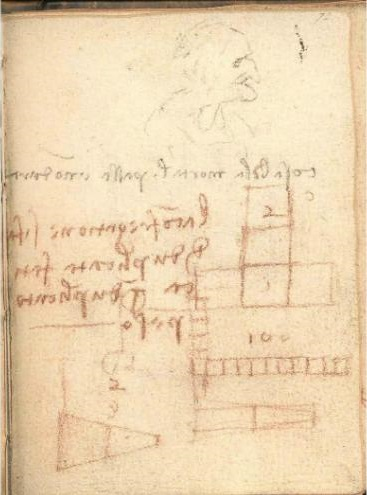
\includegraphics[width=0.45\textwidth]{Photos/LeonardDeVinci_friction_1}\hspace{0.5mm}
\end{center}
\caption{Archives des travaux de Leonard De Vinci : a) ;b) .}
\label{LeonardDeVinci}
\end{figure}
Charles August Coulomb (1736-1806)  

\begin{itemize}
\item La force de frottement statique est proportionnelle à la charge (lois d’Amontons);
\item La force de frottement statique est indépendante de la surface de contact apparente (lois d’Amontons);
\item La force de frottement cinétique (en mouvement) est indépendante de la vitesse (La loi de Coulomb).
\end{itemize}

F. Philip Bowden and David Tabor (1950) - Contact entre deux solides n'a lieu que sur des zones ponctuelles, la pression élevée sur ces points de contact qui induit une déformation plastique. Plus la pression augment plus il y a d'aspérité en contact. Les force de friction est donc dépendant de la vraie surface de contact.

\url{http://www.tribology-abc.com/}
\url{https://www.canal-u.tv/video/universite_de_tous_les_savoirs/la_tribolo-gie.1457/}

...énoncer les formules générales...

\subsection{Cas de la peau}
\subsubsection{Modèle général}
Mécanisme d'adhésion pour un polymère organique :
(équation 2.1)
\textit{F} : force de friction; \textit{Tau} : force de cisaillement ; \textit{A} : Aire de contact.

Transition thermique d'un polymère typique : (gauche: froid ; droite: chaud)
État vitreux -- \textit{Glassy state} => État visco-élastique -- \textit{Viscoelastic state} (=> État mélangé -- \textit{Melt state}) 

Pour un polymère organique dans son état vitreux, la force de cisaillement augmente linéairement avec le pression moyenne en contact, \textit{p} :
(équation 2.2)
avec \textit{tau0} la valeur intrinsèque de \textit{tau} avec pression nul; \textit{alpha} le coefficient de pression.
Or, \textit{P=W/A}
avec \textit{W} la force normale (habituellement on utilise \textit{Fn}.
 
Pour un contact entre deux corps parfaitement lisses, ici une sphère de rayon R et un plan, l'équation de hertz nous permet de déduire l'équation suivante:
(équation 2.4)

Équation de hertz permet de calculer l'intégrale du profile de pression. E : module de young, propriété du matériaux, représente l'élasticité de celui-ci. Permet de déterminer la déformation pour une contrainte donnée --- lois de Hooke. Mu : coefficient de poison intrinsèque au matériaux. rapport de la contraction transversale unitaire sur allongement axiale unitaire.

Modèle utilisable dans les deux sens: doigt/surface et point/peau. Le doigt peut aussi être assimilé à une ellipse avec R=(R'R'')...

\subsubsection{Caractérisation de l'aire de contact de bout du doigt}

Il est habituel de mesurer deux paramètres: 
\begin{itemize}
	\item \textit{Agross} Aire de contact totale (aire de contact réelle + aire des surfaces pas en contact entre les stries)
	\item \textit{Aridge} Aide de contact due aux des stries
	(\item \textit {A} aire de contact réelle
\end{itemize}
 \$Agross>Aridge>=A\&
 
 Grosse déformation de la peau dépend principalement du tissu le plus mous de la peau.
 
 Peau sèche : Aire calculé sera bien plus grande que le contact réel.
 
\paragraph{État nominal sec}
 
 Stratum coreum se comporte comme un polymère organique hydrophobe vitreux, e.g. Nylon, Keratin. Pas d'occlusion. 
 Caractéristique de ces polymères : F augmente avec l'absorption de l'humidité bien que \textit{Tau} diminue. Plastification due à l'humidité réduit le module de Young, donc d'aprés 2.4 A augmente (si on reste dans un modéle de sphére et surface parfaite).
 
 Nylon plastification augment la friction d'un facteur 2 (\textit{from dry to the satured wet states}. Au poignet augmentation d'un ordre. Cette diff vient de de la sensibilité à l'humidité du stratum coreum, qui modifie le modifie son module de Young. Conduisant à une augmentation de A (due à l'aplatissement des aspérités sous la force normale appliqué).
 
\paragraph{cas pour le bout du doigt}
 
 État mouiller: une augmentation de F  a aussi été observé. Il est supposé que A augmente vers Aridge. 
 De sec à mouiller: E de stratum coreum diminue de 3 ordre -- correspondant à une transition d'un état vitreux à un état visco-élastique. 
 
Remarque: Hydrophobie de la peau -- angle de contact de 100 degré.

Observé communément que F pour le bout du doigt augmente lorsque Fn diminue, dans le cas de charge faible, inférieur à 3,5 N. D'après (2.1)(2.2) et (2.4), on a : 
F= ... (équation 2.5)

Approximé par :
F = ... (équation 2.6)
avec n index de charge de friction; K2 coef de friction dépend de la charge

donc coef de friction, mu, vaut :
(équation 2.7)

...


Déformation du bout du doigt est bien plus complexe que le poignet (dont on a calculé le coef de friction)
 
2N déformation limite du bout du doigt due au fait que le tissu underlying est compressé contre les phalanges.

\subsection{Discussion}

Les équation de hertz ne sont pas applicable à chaque fois. Adams, Warman sont d'accord que la suggestion de Wolfman est incorrect (et bam dans les dents). Suggestion de wolfman : la friction de la peau pourrait être décrite par un coef de friction indépendant de la pression. Suggestion incorrect car le modèle prédis un indice de charge de 2/3.
Il est difficile de distinguer les eq (2.8) et (2.6) car erreur dans les données, les données sont rare en particulier lorsque le charge est faible. 

\end{document}
